%template: https://www.sharelatex.com/templates/58d81eaaca5a6fd13992f8a4
\documentclass[12pt,letterpaper]{article}

\usepackage{cvpr}
\usepackage{times}
\usepackage{epsfig}
\usepackage{graphicx}
\usepackage{amsmath}
\usepackage{amssymb}
\usepackage[style=numeric]{biblatex}
\addbibresource{references.bib}
\usepackage{csquotes}
\usepackage{caption}
\usepackage{python_code}
\usepackage{enumitem}   
% Include other packages here, before hyperref.

% If you comment hyperref and then uncomment it, you should delete
% egpaper.aux before re-running latex.  (Or just hit 'q' on the first latex
% run, let it finish, and you should be clear).
\usepackage[breaklinks=true,bookmarks=false]{hyperref}
\usepackage[title]{appendix}
\usepackage{xcolor}
\newcommand\myworries[1]{\textcolor{red}{#1}}

\cvprfinalcopy % *** Uncomment this line for the final submission

\def\cvprPaperID{****} % *** Enter the CVPR Paper ID here
\def\httilde{\mbox{\tt\raisebox{-.5ex}{\symbol{126}}}}

\linespread{1.5}
\setlength{\parindent}{2.5em}


% Pages are numbered in submission mode, and unnumbered in camera-ready
%\ifcvprfinal\pagestyle{empty}\fi
\setcounter{page}{1}
\begin{document}

%%%%%%%%% TITLE
\title{\textbf{ESC499 Interim Report:\\ \textit{Profiling GPU Memory with PyTorch}}}

\author{Author: Izaak Niksan\\
%Department of Computer Science, University of Toronto\\
%{\tt\small izaak.niksan@mail.utoronto.ca}\\
Supervisor: Prof. Gennady Pekhimenko\\
Advisor: Hongyu Zhu
}

\maketitle
%\thispagestyle{empty}
\newpage
%%%%%%%%% INTRODUCTION
\section{Introduction}
Deep neural networks (DNNs) have a history dating back over half a century, with Donald Hebb's \enquote*{Hebbian Learning Rule} laying the foundations for modern techniques \cite{dnn_history}. In the proceeding years this approach was developed and improved, with notable developments by Rosenblatt (the first perceptron), Werbos (backpropagation), Jordan (Recurrent Neural Network), Hochreiter \& Schmidhuber (LSTM), and Hinton (Deep Belief Networks) \cite{dnn_history}. While this theoretical progression was occurring, the computational machinery required to actually implement these models was non-existent. In the last decade, the development of high-performance computing hardware - especially GPUs - has enabled many of these once-theoretical DNNs to be implemented in practice. Still, however, there remain bottlenecks which constrain implementations and therefore deeper insight into underlying resource usage is vital for further advancements in the field. Of these resources, GPU memory is among the most important to understand given its scarcity. \par 

\section{Background}
%%%%%%%%% BACKGROUND::Neural Networks
\cvprsubsection{Neural Networks}
While there are many types of artificial neural networks, they all involve the transformation of some input data (for example the pixels of an image) into meaningful output - in fact, a neural network is nothing more than a composition of mathematical functions. The function modeled by a neural network is special, however, because it can model \textit{any} mathematical function with arbitrary accuracy (provided that the network has at least two layers) \cite{dnn_history}. It is because of this property that neural networks have been labeled \enquote*{universal approximators}. Loosely, this means that if there are useful patterns in the world - whether they correspond to user preferences in movies based on past movies they have watched, or classification of images based on their pixel composition, or even cardiac arrest likelihood based on heart rate - a sufficiently-trained neural network can identify it. The effectiveness of a neural network in identifying these patterns depends primarily on two things: the amount of data it has been trained with, and its specific topology.
\par

\begin{figure}[h]
\centering
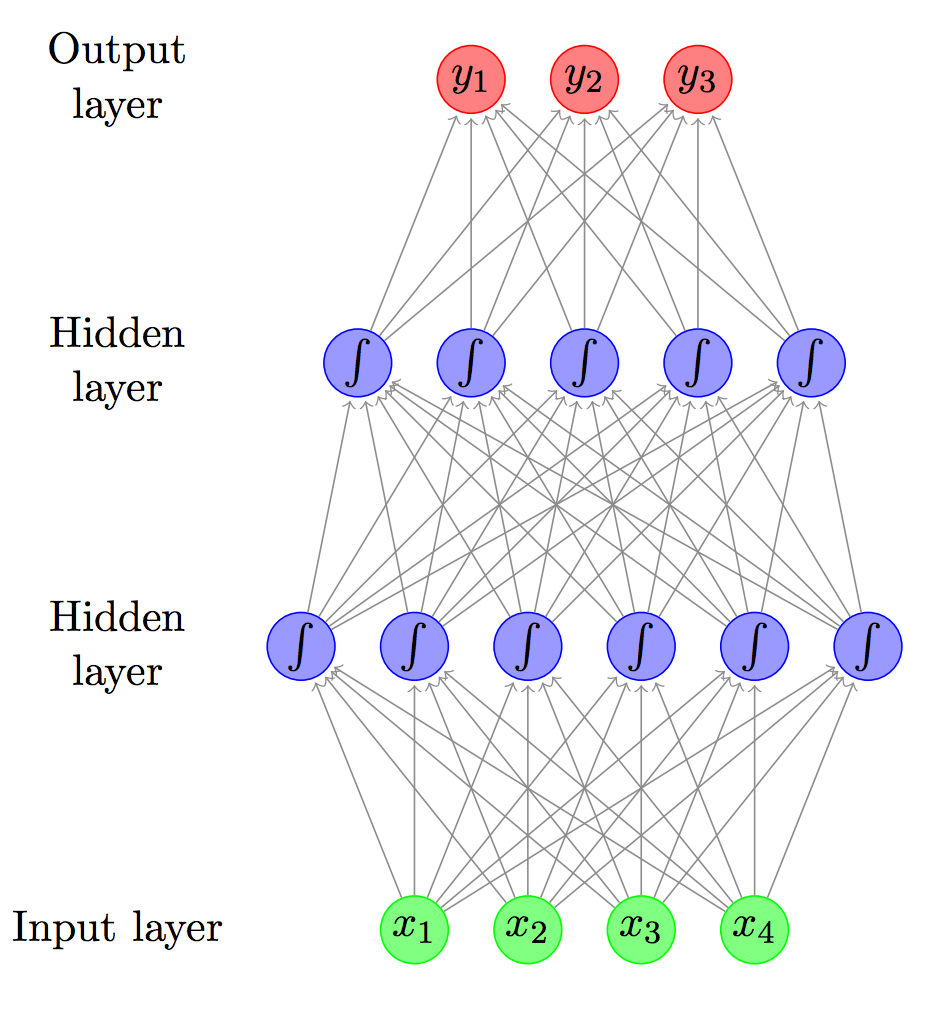
\includegraphics[width=0.4\textwidth,height=9cm]{neural_network_machinelearningmastery.png}
\captionsetup{width=0.7\linewidth}
\caption{ Topology of a fully-connected feedforward neural network \cite{feedforward_pic}}
\label{fig:feedforwardNN}
\end{figure}

The neural network in Figure \ref{fig:feedforwardNN} shows the basic building blocks from which modern neural networks emerge. It is a simple feedforward neural network - a more complete list of network types can be found in Appendix \ref{appendix:types_of_networks}. The green nodes represent the input data to the network, which is what the network must use to make meaningful predictions. Perhaps, the input vector $[x_1,x_2,x_3,x_4]^T$ might represent a four-word sentence.\par

The gray lines in the diagram represent \textit{weights}, or the scaling coefficients from one node to the next. These weights together create linear combinations of the outputs of one layer into the nodes of the next layer. \par 

The purple nodes represent \textit{neurons}, which take a weighted sum of input nodes and produce a scalar-valued output. Each neuron is a nonlinear function; the nonlinearity is important here because without it the universal approximator guarantees no longer apply. For example, each neuron might be the ReLU function $f(x)=max(x,0)$ which clips all negative values. The intermediate outputs of each layer are known as \textit{feature maps}. Notice how there are two layers of purple nodes here - this denotes that the model has two hidden layers. There can be an arbitrary number of hidden layers in a network, and while there is no standard for the number of layers required for a network to be considered a \enquote*{deep neural network}, it should have at least three. \par 

Finally, the red nodes are the \textit{outputs}, which are the network's predictions based on the provided input data. In this example, each output node might be the one-hot-encoded representation of who likely wrote the input sentence. The result closest to 1 here indicates a network's predicted output node. If $y_1$ is associated with Alice, $y_2$ with Bob, and $y_3$ with Charlie, then the output vector $[y_1,y_2,y_3]^T = [0.983,0.217,0.015]^T$ indicates that it was likely Alice's sentence.

%%%%%%%%% BACKGROUND::GPUs and their application to DNNs
\cvprsubsection{GPUs and Their Applications to DNNs}
Graphics Processing Units (GPUs) are at the center of recent machine learning breakthroughs. It turns out that the computational workloads of neural networks are, in essence, sequences of matrix operations; as it was shown in the previous section, matrix multiplication is used to conveniently denote the application of scalar weights to the output of a neural network layer. GPUs can perform these computations orders of magnitude faster than CPUs due to the parallelism inherent in their design.  Figure \ref{fig:turing} shows the architecture of a modern GPU, which contains numerous computational cores (green).

\begin{figure}[h]
\centering
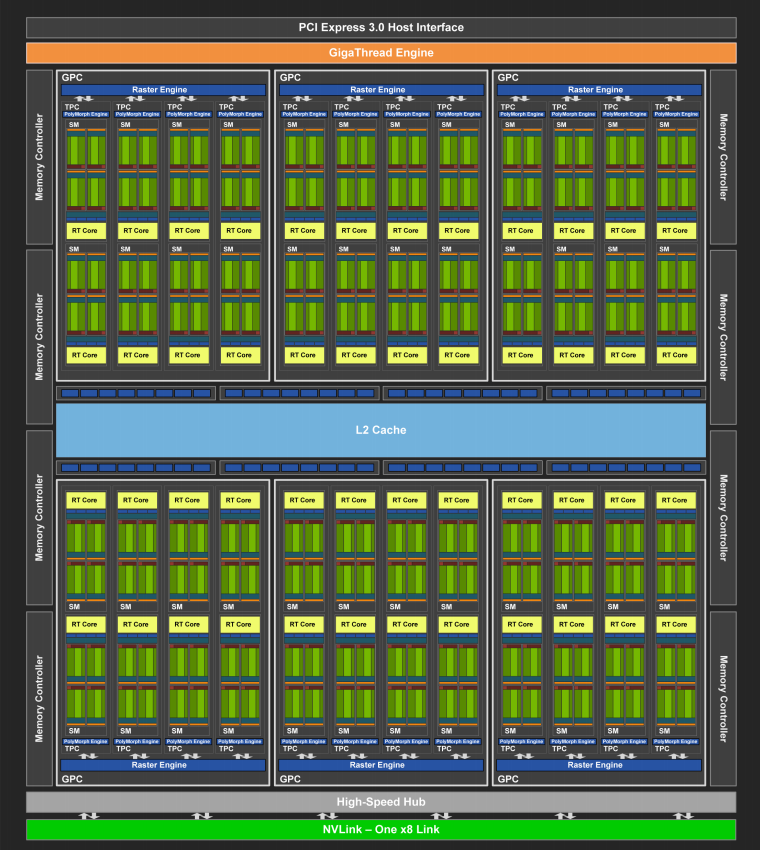
\includegraphics[width=0.6\textwidth]{Turing_TU104_chip_diagram.png}
\captionsetup{width=0.8\linewidth}
\caption{Diagram of the NVIDIA Turing TU104 architecture. Green sections are CUDA cores, which together compose Streaming Multiprocessors (SMs) \cite{turing_architecture}}
\label{fig:turing}
\end{figure}

To understand the value that GPUs bring in terms of computational parallelism, suppose that a simple program is scaling a matrix as follows:
\[
3
\begin{bmatrix}
    a  &  b      \\
    c  &  d      
\end{bmatrix} 
=
\begin{bmatrix}
    3a  &  3b      \\
    3c  &  3d      
\end{bmatrix} 
\]
This computation can be distributed over 4 GPU cores, which would each scale one element of the matrix. The program can then accumulate the results of the four operations, and store the results either by overwriting the old matrix or by creating a new one in memory. While this is a small example, the same principles can be applied to matrices with thousands of elements - as the dimensions increase, so does the benefit of using GPUs. 
\par

NVIDIA conveniently provides the functionality to distribute a program's workload across GPU cores in the form of a rich C++ API \cite{cuda_guide}. This API can be integrated seamlessly into existing codebases in such a way that the programmer is abstracted away from the low-level architecture of the GPU they are using. In recent years, highly-tuned primitives for machine learning-specific applications (e.g. convolution, softmax, batch normalization, neuron activations, etc.) have become publicly available \cite{cudnn}, which further allow programmers to use GPUs to their benefit.
\par 

%%%%%%%%% BACKGROUND::Inference and Training
\cvprsubsection{Inference and Training}
Neural networks are used in two modes: \textit{training} and \textit{inference}. While these two modes are closely related, they have certain key differences which ultimately affect the way they each interact with GPUs. A useful neural network must first be trained - this process involves iteratively improving the network's trainable parameters (i.e. weights) which are either initialized randomly or all to zero. Training can further be broken down into two steps: a \textit{forward pass} and a \textit{backward pass}. As it turns out, the forward pass is very similar to inference. Thus, the training of a neural network can be thought of as an extension of the inference process.
\par 

Both inference and the forward pass of training accept some input data (in the Figure \ref{fig:feedforwardNN} example this would be $[x_1,x_2,x_3,x_4]^T$). These input nodes are passed through the network - whatever its specific topology may be - and transformed through compositions of weight scaling and nonlinear activation functions. Then, at the end of the network the outputs are produced. For inference, these final outputs are almost always the only thing that the user is interested in, since they are the meaningful interpretations of the input data. For the forward pass of training, however, more than just the final outputs must be kept; in fact, nearly all of the intermediate values that were used to propagate the data through the network must be kept for later stages of the training algorithm.
\par

%%%%%%%%% BACKGROUND::Backpropagation and Memory
\cvprsubsection{Backpropagation and Memory}
Once the forward pass of training has finished, the first step is to evaluate the outputs of the network based on how accurate their predictions were. These evaluations are done via a \textit{loss function}, which quantifies the difference between the network's outputs and the \textit{ground truth} of the input data (in most cases this refers to the \textit{correct} interpretation of the input data). Referring once again to the previous example, if it was known that Bob in fact wrote the sentence, then the network's output $[y_1,y_2,y_3]^T = [0.983,0.217,0.015]^T$ would be compared to the ground truth $[0,1,0]^T$ and produce a large loss function result, since $y_2$ was not close to 1 and $y_1$ was incorrectly close to 1. While loss functions are beyond the scope of this paper, more information on them can be found in Appendix \ref{appendix:types_of_loss_functions}.
\par

Next comes perhaps the most important part of training - backpropagation. Originally gaining traction in the late 1980s \cite{hinton_backpropagation}, backpropagation involves calculating the partial derivatives of the loss function with respect to each weight in the network by using the chain rule. These calculations require the intermediate outputs of each layer, which are generally kept in memory during the forward pass and held until they are needed. Once all the gradients in the network have been calculated, they can then be adjusted appropriately. It is this extra space requirement that lies at the heart of why GPU memory is an essential resource. As for how the weights are updated, there are many different algorithms known as \textit{optimizers} available \cite{optimizers} which can be employed. Gradient Descent, perhaps the most ubiquitous optimization algorithm, is known as a first order optimization algorithm. It involves updating each weight in the network by a global scaling factor after all the gradients have been computed. Another popular algorithm is Adam \cite{adam}, which is known as a second order algorithm. Once again, the exact details of such algorithms are beyond the scope of this paper.
\par

Generally the training process is done with a training dataset, which should be an unbiased representation of what actual data looks like in the real world. For example, it is important that a speech to text model is not trained using only the speech of one person, otherwise the network would learn to recognize \textit{their} speech very well but would likely under perform when fed data from another person's speech. Training datasets are generally very large - for example, a commonly-used object detection dataset known as COCO \cite{COCO} has 330 000 images, and is 37.57 GB in size. This is far beyond the size of a typical GPU's memory. One implementation of Gradient Descent involves using mini-batches, which are uniform-size subsets which together comprise the entire dataset. Each example within a mini-batch has the training algorithm applied to it, and only once the entire mini-batch is completed are the weights updated based on the sum of all gradients. A breakdown of the entire training process is summarized in Figure \ref{fig:training_memory_breakdown}.
\par

\begin{figure}[ht]
\centering
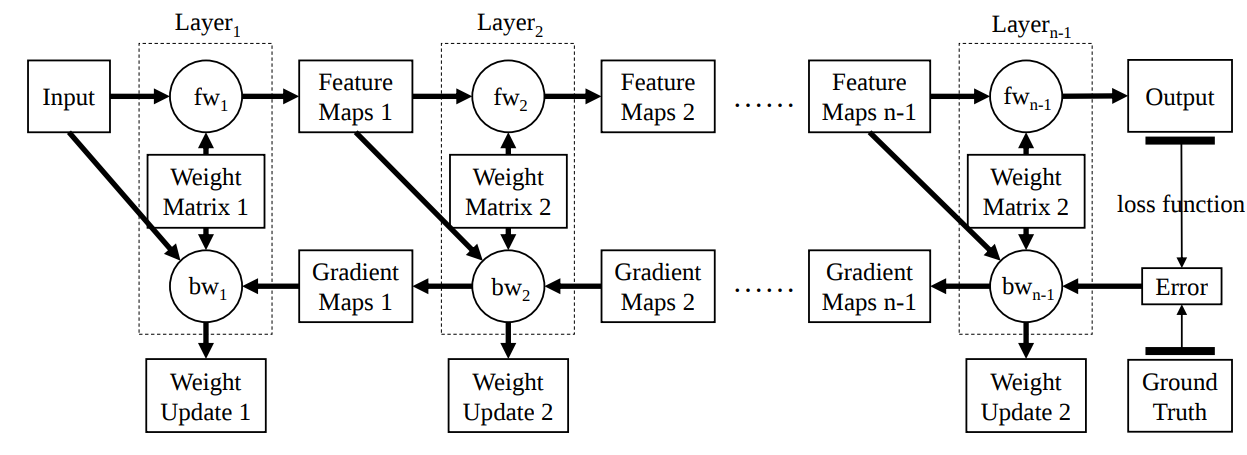
\includegraphics[width=1\textwidth]{training_memory_breakdown.png}
\captionsetup{width=0.7\linewidth}
\caption{A breakdown of the training process, courtesy of TBD \cite{tbd}}
\label{fig:training_memory_breakdown}
\end{figure}

%%%%%%%%% BACKGROUND::Machine Learning Frameworks and Memory Profilers
\cvprsubsection{Machine Learning Frameworks and Memory Profilers}
\label{sec:Machine_Learning_Frameworks_and_Memory_Profiler}
In practice, DNNs are implemented via frameworks such as  Caffe \cite{caffe}, Theano \cite{theano}, MXNet \cite{mxnet_paper}, TensorFlow \cite{tensorflow}, CNTK \cite{cntk}, Chainer \cite{chainer}, Torch \cite{torch}, Keras \cite{keras}, and PyTorch \cite{pytorch_paper}. These frameworks provide convenient interfaces which enable researchers to codify their DNN architecture in common programming languages including Python, C++, and Java. Despite the rise in popularity of these frameworks in recent years, comprehensive tools to understand their memory usage are not provided out of the box. The EcoSystem research team at UofT, led by Prof. Gennady Pekhimenko, has recently developed open-source memory profiling tools for MXNet \cite{mxnet_paper}, TensorFlow \cite{tensorflow}, and CNTK \cite{cntk}; such a tool for PyTorch, however, remains to be created. PyTorch is increasingly becoming one of the most widely-used frameworks and thus a memory profiler would have a large impact to the community.
\par

All of these machine learning frameworks employ directed acyclic \textit{computational graphs}, which organize sequences of operations on data. The nodes of computational graphs are the program's variables (tensors, scalar values, etc.), while the edges represent data dependencies. Edges terminating at a node signify inputs to a certain mathematical function, whose output value is stored in the variable representing the node. For the purposes of backpropagation, each node must also know how to compute the derivative of its output with respect to its inputs. In Figure \ref{fig:computational_graph}, the green edges represent the flow of data in a forward pass. Once the output $e$ has been calculated, the backward pass can be initiated, during which the gradients are calculated by traversing the graph in the reverse direction (red edges).
\par 

\begin{figure}[ht]
\centering
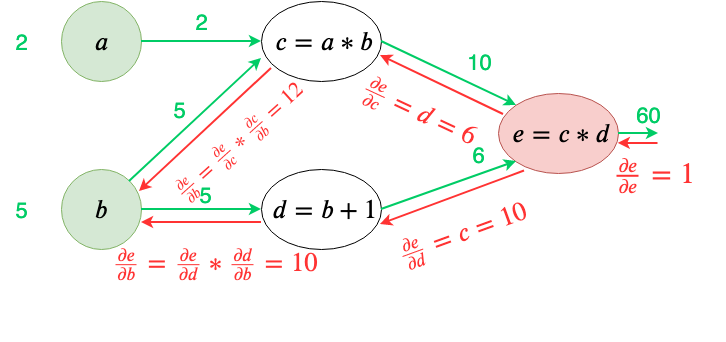
\includegraphics[width=.7\textwidth]{computational_graph_example.png}
\captionsetup{width=0.7\linewidth}
\caption{A simple computational graph \cite{computational_graph_example} which calculates $\frac{\partial e}{\partial b}$}
\label{fig:computational_graph}
\end{figure}

The frameworks that these memory profilers were created for all use static computational graphs. MXNet, for example, allows users to define computational symbols in their front end language which are then compiled under the hood. Since this graph is defined at the start, the program does not need to wait until the forward pass to create the graph. This compiled graph contains all placeholders for input and output tensors. When it comes time to use the graph - i.e. pass some input data through the network in the forward pass - MXNet internally calls its \textit{executor} \cite{mxnet_executor}. The executor will then allocate the memory for the tensors required for the graph. This point is important because specific memory regions of the GPU are linked to parts of the computational graph, and remain linked for the duration of the program. To derive meaning from what each part of the computational graph does - for example the part of the graph representing a Long Short-Term Memory (LSTM) cell \cite{lstm} within a speech recognition model - the naming employed by the programmer is used. Listing \ref{listing:lstm_example} shows an example of how a programmer might define an LSTM cell in their code. Notice the name assignments that are inputted as function parameters - i2h meaning \enquote{input to hidden} and h2h meaning \enquote{hidden to hidden} - which are meaningful descriptors of the neural network's layers.

\begin{lstlisting}[language=Python, caption={Symbolic naming of an LSTM cell, taken from the MXNet GPU profiler documentation \cite {mxnet_profiler}}, label={listing:lstm_example}]
i2h = symbol.FullyConnected(data=inputs, weight=self._iW, bias=self._iB,
                            num_hidden=self._num_hidden*4,
                            name='%si2h'%name)
h2h = symbol.FullyConnected(data=states[0], weight=self._hW, bias=self._hB,
                            num_hidden=self._num_hidden*4,
                            name='%sh2h'%name)
\end{lstlisting}

Thus, the picture so far is that a user defines their network and training/inference procedures in a front end language such as Python, using existing machine learning framework APIs. This framework interprets the user's code, and distributes the computational work to one or more GPUs (CPUs can be used as well, but for reasons outlined earlier GPUs are preferred). There are APIs used by the framework to interact with the GPU, which may vary as well. For NVIDIA GPUs, CUDA APIs are used, which interact with C++, C, and Fortran. For this reason, along with the fact that interpreted languages such as Python are generally less efficient than compiled languages, machine learning frameworks are themselves primarily written in C or C++.
\par 

For the purposes of this paper, one CUDA function is of particular importance: \texttt{cudaMalloc()}. This function allows the framework to request any number of bytes in memory on the device\footnote{Typically, \textit{device} refers to the GPU and \textit{host} refers to the CPU}. Each call to \texttt{cudaMalloc()} will return a pointer to where the requested memory lies; if space for a tensor was requested, then this pointer might be used for the remainder of the program to access and modify this tensor. However, it is ultimately up to the framework to manage its memory, and different frameworks have different strategies. 
\par 

The MXNet memory profiler's main challenge is linking symbol names to specific \texttt{cudaMalloc()} calls. This linkage allows the profiler to establish how much memory was needed for which part of the computational graph, and therefore can determine the memory breakdown of the models' weights, activations, and gradients. However, there is no direct way to do this in the existing MXNet codebase, and thus it was modified to make these connections. Function signatures were changed so that the strings representing symbol names could be passed down to the underlying allocations. A C++ helper class was created to output entries into a log file with information about the memory breakdown. The log file can then be parsed with provided scripts to create visualizations of the results.
\par 

\begin{figure}[ht]
\centering
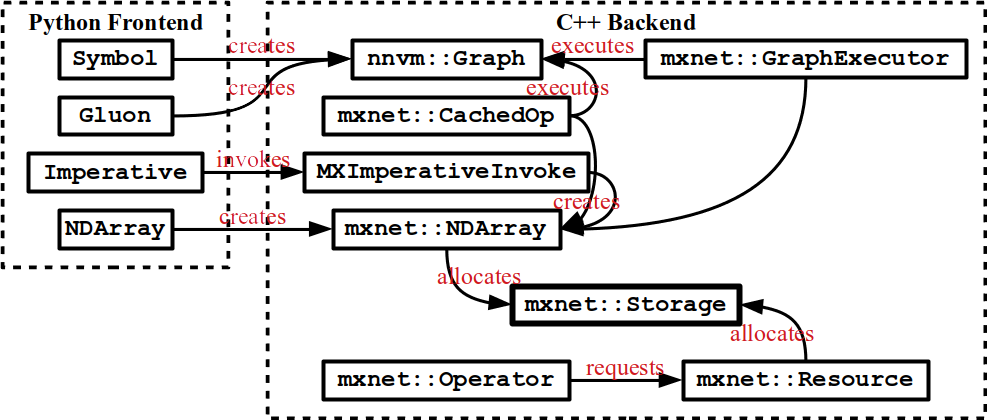
\includegraphics[width=.8\textwidth]{mxnet_profiler_design.png}
\captionsetup{width=0.7\linewidth}
\caption{MXNet GPU Profiler system design \cite{mxnet_profiler}}
\label{fig:mxnet_design}
\end{figure}

%%%%%%%%% PROGRESS TO DATE
\section{Progress to Date}
\label{progress_to_date}
Unlike the frameworks for which these memory profilers were created, PyTorch uses completely different memory management and computational graph strategies. In order to create a memory profiler for PyTorch, these differences must be investigated and thoroughly understood. This involves investigating both its front end (Python\footnote{While PyTorch does have a C++ front end as well, it is generally less user-friendly and not used as often}) and back end (C++) code implementations. This section discusses the internals of PyTorch and how a memory profiler can be created.

%%%%%%%%% PROGRESS TO DATE::Memory Caching
\cvprsubsection{Memory Caching}
\label{sec:memory_caching}
The first difference - and perhaps most important one in the context of this paper - is how PyTorch handles its device memory. Unlike other frameworks, PyTorch uses \textit{caching} as its primary memory management strategy. The reason for this lies in the fact that PyTorch does not create a static computational graph with pre-allocated room for variables and tensors. This new paradigm, which is discussed in later sections of this paper, is known as \textit{dynamic computational graphs}. For now it suffices to say that PyTorch does not know how the forward and backward pass will be executed until runtime, i.e. until training or inference begins. Caching is best explained by the creators of PyTorch \cite{pytorch_paper}:

\begin{quote}
\enquote{
PyTorch implements a custom allocator which incrementally builds up a cache of CUDA memory and reassigns it to later allocations without further use of CUDA APIs. The incremental allocation is also crucial for better interoperability, because taking up all GPU memory ahead of time would prevent the user from utilizing other GPU-enabled Python packages. To further improve its effectiveness, this allocator was tuned for the specific memory usage patterns of deep learning. For example, it rounds up allocations to multiples of 512 bytes to avoid fragmentation issues. Moreover, it maintains a distinct pool of memory for every CUDA stream (work queue).
}
\end{quote}

By incrementally creating a cache of memory as-needed during runtime, PyTorch does not need to make frequent \texttt{cudaMalloc()} calls to reserve space for each tensor as the forward or backward pass progress. Instead, it reserves chunks of space which can be assigned and unassigned freely by PyTorch. The allocation strategy is relatively straightforward: when a tensor is needed by the program, it can request space for it using an allocator. If there is enough space in the existing cache, it takes memory from there. If not, the cache size is increased, and then the tensor is assigned memory from the cache. For Cuda, \myworries{Allocator interface code, CUDACachingAllocator, line number of code}.
\myworries{Example of memory size calculation: numel*...}
\par 

In general, deallocation strategies are more nuanced than their allocation counterparts. There is no reason for a tensor to occupy space in device memory if the tensor is no longer being used by the program. Other machine learning frameworks generally use \textit{garbage collection} techniques to free memory once it is no longer needed. With this technique, the program will periodically analyze the state of all objects in its memory. Every object currently in use - i.e. tensors that are needed for future computations - is marked. The garbage collector will then free all objects in its address space that are not marked; these objects are of no use to the program. The issue with garbage collection is the timing of the collection - for the duration between a tensor becoming unneeded and garbage collection occurring there is wasted device memory.
\par 

PyTorch does not use garbage collection. Instead, to determine whether a certain tensor is needed or not, a technique called \textit{reference counting} is employed. The reference counter of a tensor is modified dynamically at runtime based on how many variables reference it. This system tracks both the back end references (PyTorch's internal references to the tensor) as well as the front end references (user-created references in their Python code) to ensure that a tensor is only freed when there is truly no use for it anymore. When a reference counter reaches zero, the memory occupied by the tensor is immediately released back to the cache. This means that at no point will there be objects with zero references which still occupy device memory. It should be noted here that the program's cache size generally does not decrease - thus even when the reference counting system frees a tensor, the total device memory occupied by the PyTorch program will not decrease since it is still held by the cache.
\par 

By gradually increasing the cache size as the program progresses, the majority of the CUDA memory API calls will occur near the start of the program, particulary in the first few iterations\footnote{An iteration refers to the combined forward and backward pass of one mini-batch through the network} of training. This is illustrated in Figure \ref{fig:cuda_memory_kernels}, where the utilization of the GPU (density of CUDA kernel execution in blue) is low in the first iteration compared to subsequent iterations. This decreased computational efficiency can be attributed to the costly memory management APIs.
\myworries{example of memory usage graph, allocated vs max allocated? also talk about nvidia-smi}

\begin{figure}[ht]
\centering
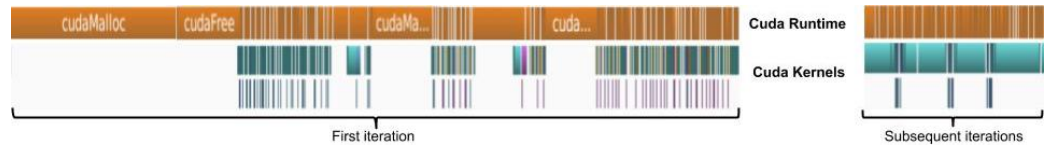
\includegraphics[width=.9\textwidth]{cuda_kernel_caching.png}
\captionsetup{width=0.7\linewidth}
\caption{ResNet-50 GPU execution traces in PyTorch \cite{pytorch_paper}}
\label{fig:cuda_memory_kernels}
\end{figure}

 
%%%%%%%%%%%%%%%%%%%%%%%%%%%%%%%%%%%%%%%%%%%%%%%%%%%%%%%%%%
%
%     PROGRESS TO DATE::Tensors in PyTorch
%
%%%%%%%%%%%%%%%%%%%%%%%%%%%%%%%%%%%%%%%%%%%%%%%%%%%%%%%%%%

\cvprsubsection{Tensors in PyTorch}
\label{sec:tensors_in_pytorch}
Thus far, tensors have been mentioned but not yet explained in detail. Tensors are n-dimensional data structures which contain a certain type of data, for example integers or floats. The actual data represented by a tensor - for example a matrix representing the scalar weights from the first to the second hidden layer of a network - is accompanied by some metadata which describes various attributes about the tensor. The metadata of a tensor includes its dimensions (depth, height, width), strides, element data type, and the device it is stored on. Among these, strides may be an unfamiliar one - in fact, striding is one of the defining features of PyTorch. To explain striding, it must first be understood that every tensor is associated with a \textbf{storage} object. A tensor can be thought of as the logical view of data, while a storage can be thought of as a structure which manages the raw data. It is entirely possible in PyTorch for two tensors to point to the same storage object, with each of the two tensors having different perspectives about how to view the underlying raw data. For example, suppose a PyTorch program created the following two tensors:

\[
X =
\begin{bmatrix}
    1      \\
    2      \\
    3      \\
    4      \\
\end{bmatrix} 
,
Y =
\begin{bmatrix}
    1  &  2      \\
    3  &  4      
\end{bmatrix} 
\]
Both $X$ and $Y$ contain the integers from 1 to 4; however, they each provide different logical representations of the data. This information is captured by the stride of a tensor, which are offsets to map element indices into specific memory addresses. Storages don't understand the data they encapsulate, it is up to the tensors to provide the interpretation. The reference counters explained in section \ref{sec:memory_caching} are in fact handled by storage objects. When no tensors point to a certain storage anymore, the memory occupied by the storage is release to the cache.  
\par 

Given that this paper is concerned with the memory usage of PyTorch, two questions must be answered: \myworries{answers are  data ptr, numel*}
\begin{enumerate}[label=(\roman*)]
  \item How can a tensor abstraction's link to underlying device memory be ascertained, and how can a memory profiler safely handle two or more tensors which point to the same underlying storage?
  \item Given (i), how can this link be translated into a specific size in bytes, and how can a memory profiler take into account PyTorch's unique caching memory management strategy, where CUDA memory allocations are no longer directly tied to a specific object within the framework?
\end{enumerate}

%%%%%%%%%%%%%%%%%%%%%%%%%%%%%%%%%%%%%%%%%%%%%%%%%%%%%%%%%%
%
%     PROGRESS TO DATE::Models in PyTorch
%
%%%%%%%%%%%%%%%%%%%%%%%%%%%%%%%%%%%%%%%%%%%%%%%%%%%%%%%%%%

\cvprsubsection{Models in PyTorch}
\label{sec:models_in_pytorch}
Tensors can only get a user so far. Ultimately, machine learning researchers need an interface to codify their machine learning models, which can then be trained and used. The main interface used to do this in PyTorch is the \texttt{nn.Module} class. For example, Listing \ref{listing:nn.module_example} defines a simple two-layer network:
\par 
\begin{lstlisting}[language=Python, caption={Definition of a simple two-layer neural network from the PyTorch documentation \cite{pytorch_tutorial}}, label={listing:nn.module_example}]
class TwoLayerNet(torch.nn.Module):
    def __init__(self, D_in, H, D_out):
        super(TwoLayerNet, self).__init__()
        self.linear1 = torch.nn.Linear(D_in, H)
        self.linear2 = torch.nn.Linear(H, D_out)

    def forward(self, x):
        h_relu = self.linear1(x).clamp(min=0)
        y_pred = self.linear2(h_relu)
        return y_pred
\end{lstlisting}
Here, a network called \texttt{TwoLayerNet} is being defined. Notice how it inherits from \texttt{nn.Module}. The \texttt{\_\_init\_\_} method of this network is invoked whenever an instance of it is created and a user generally instantiates one model which persists for the duration of their PyTorch program. This method is where the \textit{structure} of the model is defined - how many and what types of layers are present, which layers connect to what, and so on. The code here can be as complex or as simple as the user wishes; this modularity is what enables PyTorch to implement arbitrary neural networks. This example creates two linear layers using the PyTorch-provided \texttt{torch.nn.Linear} \footnote{The \texttt{torch.nn.Linear} layer applies the linear transformation $y=xA^T + b$} implementations \cite{pytorch_docs}. The input parameters \texttt{D\_in} and \texttt{D\_out} are used to specify the dimensions of these two layers.
\par 

One interesting feature of the \texttt{\_\_init\_\_()} method is that all \textit{learnable} layers of the network - i.e. ones that must be trained, which must have their gradients computed - are automatically registered and saved to the model's list of \texttt{parameters}. Using the \texttt{torch.nn.Linear} API handles this by default, but if one were to define a learnable tensor themselves, they would have to wrap them with \texttt{torch.nn.Parameter}. For example, observe the following two tensor definitions: 

\begin{lstlisting}[language=Python]
import torch
class MyNetwork(torch.nn.Module):
    def __init__(self):
        super(MyNetwork, self).__init__()
        self.wont_be_registered=torch.tensor([1.0])
        self.will_be_registered=torch.nn.Parameter(torch.tensor([1.0]))
\end{lstlisting}
Here, one tensor is defined correctly and thus will forever be saved in a special data structure by the PyTorch back end code. This data structure is called the \texttt{state\_dict}. The other is not, and will not be added to the \texttt{state\_dict}. Wrapping a tensor in this way does not change any of its functionality. To verify that tensors are being saved as expected, an instance of the model is instantiated and then a built-in class function called \texttt{named\_parameters()} is invoked to reveal the named items within the model's \texttt{state\_dict}:
\begin{lstlisting}[language=Python]
model=MyNetwork()
for name,param in model.named_parameters():
    print(f"Tensor name={name}, Tensor data={param}")
\end{lstlisting}
The output is as follows:
\begin{lstlisting}[language=Python]
>>> Tensor name=will_be_registered, Tensor data=Parameter containing:
    tensor([1.], requires_grad=True)
\end{lstlisting}
\par
This convenient storage of layer names has many similarities to the one previously discussed in MXNet in section \ref{sec:Machine_Learning_Frameworks_and_Memory_Profiler}, and will serve to be useful in creating a new memory profiler for PyTorch given the mapping it provides between layer names and their data objects. 
%%%%%%%%% PROGRESS TO DATE::Dynamic Computational Graphs and Autograd
\cvprsubsection{Dynamic Computational Graphs and Autograd}
The network definition in Listing \ref{listing:nn.module_example} has one other important definition, namely its \texttt{forward()} method. This method describes the exact sequence of calculations that will be undertaken during the forward pass of the network, both during training and inference. This example is trivial, and the backward pass procedure could be defined manually with some basic calculus and a few lines of code. However, modern neural networks are very complex and have detailed computational procedures that define their forward passes. Manually defining a backward pass each time would be an arduous and error-prone process, and thus a more scalable system is required.
\par

PyTorch uses \textbf{automatic differentiation} \cite{automatic_differentiation}, implemented within the \texttt{torch.autograd} package, to take care of this problem. Distinct from other algorithmic methods such as symbolic and numerical differentiation, automatic differentiation is founded on the observation that any arbitrary computer program can be decomposed into arithmetic operations ($+,-,*,\div$) and elementary functions ($log, sine, cosine, exp,$ etc.). Recursively applying the chain rule allows the program to calculate derivatives (subject of course to floating point precision errors) using only an order of $O(n)$ extra computation. In practice, the linear factor is typically small in magnitude, leading to only a small decrease in performance.
\par 

During each iteration, PyTorch will gradually create a computational graph \textit{dynamically} as the program executes - this is a large departure from other frameworks, such as MXNet, which create a \textit{static} graph at the start of the program. When PyTorch starts the backward pass with a $.backward()$ call, the graph will be walked back and gradients will be calculated. Returning to Figure \ref{fig:computational_graph}, the gradient of the output node $e$ with respect to the input node $b$ could not be calculated directly; because of the nature of the chain rule, the gradients of \textit{intermediate} nodes were required for the calculation. These occupy space in memory and must not be neglected. Notice also that derivatives with respect to $a$ were \textit{not} calculated; for this reason, it cannot be assumed that every node will participate in PyTorch's backward pass procedure. In fact, if the gradient of $a$ with respect to the output $e$ were not required, and there were other intermediate nodes in the graph which were not needed for computing the gradient of $e$, these nodes would not have their gradients calculated either. Thus, it cannot be assumed that every tensor involved in a PyTorch computational graph will necessarily have its gradients computed and stored in memory. More generally, if a tensor has \texttt{requires\_grad=True}, then PyTorch must calculate gradients for it. The exact behaviour is outlined in the PyTorch documentation \cite{pytorch_doc_leaf_requires_grad}. 
\par 

%%%%%%%%% PROGRESS TO DATE::Gradients, Activations, and Hooks
\cvprsubsection{Activations, Gradients, and Hooks}
Activations are the scalar outputs of network layers, and gradients are the derivatives necessary for backpropagation. To create a memory profiler, the tensors which represent these data structures must be properly accounted for. During the forward pass of training, activations are gradually computed and stored in PyTorch's memory cache. Then, during the backward pass, gradients are computed using these activations. Immediately after the backward pass, all of these intermediate tensors are no longer needed, and are cleared from the cache. At this point, only the gradients of \textbf{leaf tensors} \cite{pytorch_doc_leaf_requires_grad} of the computational graph - i.e. the ones ones which must be improved during the iteration - are kept in memory. These gradients can then be used by an optimizer (e.g. Adam) to take a step in the direction which reduces the loss function of the network.
\par 

This complicated set of procedures - where the total allocated memory routinely fluctuates throughout training, and where tensor memory is not even linked directly to \texttt{cudaMalloc()} calls but rather is simply taken and returned to a global cache - provides new challenges not faced when tracking the memory of a static graph framework. Luckily, however, PyTorch provides some hidden tools which help shed light on the forward and backward pass: \textbf{hooks}.
\par 

There are several variants of hooks in PyTorch, but unfortunately they have very little documentation. Still, the insight they bring is valuable, despite the fact that most information about them is only found spread across the PyTorch forums \cite{pytorch_forum}. Hooks are \textit{functions} which can be registered on either a \texttt{nn.Module} or a \texttt{Tensor} object. The three methods used to register hooks are: \texttt{register\_hook()}, \texttt{register\_forward\_hook()}, and \texttt{register\_backward\_hook()}. Depending on the type of hook, during the backward or forward pass these functions are called. Hooks allow direct access to the intermediate activations and gradients at the time of their creation - exactly what is needed for a memory profiler.  %Further complicating things, the behaviour of hooks differs depending on whether they are registered to a \texttt{nn.Module} or a \texttt{Tensor}.
\par 




%The \texttt{.grad} attribute of a tensor stores its gradient 
% forward hook, backward hook
% Previously, learnable was mentioned: what does it mean


%%%%%%%%% PROGRESS TO DATE::Creating the Profiler
\cvprsubsection{Creating the Profiler}
% garbage collection? during a hook run garbage collection?
%data pointers, size of memory
In the face of all the internal complexities that have been outlined thus far, it should be clear that that new mechanisms must be created to profile PyTorch's device memory usage. A proposed strategy to attain a layer-by-layer breakdown into weights, activations, and gradients is developed using knowledge and methods that have been developed in previous sections. It is noted that this strategy departs from the strategies used with existing profilers in that it only uses the front end Python API available in PyTorch. This means that the profiler is version-agnostic and thus future-proof. Given the particularly fast-changing nature of PyTorch, with several recent large-scale design changes such as the variable-tensor merger \cite{pytorch_variable_tensor_merger}, having a profiler that does not have to be re-coded each time a new update arrives is a significant benefit. 
\par 

First, let us return to the two questions posed in section \ref{sec:tensors_in_pytorch}. Question (i) requires linking tensors to the locations of their device memory. To solve this, there is a fundamental structure in PyTorch known as a \textbf{DataPtr}. Defined in \texttt{c10/core/Allocator.h} in the source code, these structures are described as follows:
\begin{quote}
\enquote{
A DataPtr is a unique pointer (with an attached deleter and some context for the deleter) to some memory, which also records what device is for its data.}
\end{quote}
The DataPtr of a tensor is saved in the \texttt{storage} object that the tensor points to, and can be accessed by calling \texttt{tensor.storage().data\_ptr()}. This also provides a way to determine if two tensors with different names actually share the same underlying memory, and thus should not be counted twice by the profiler. A hash table which maps the layer naming of a tensor to its DataPtr can be used by the profiler to keep track of tensors. It is important that this hash table \textbf{does not store a direct reference to the tensor itself}, since this would prevent the reference counting system from freeing it as expected, and thus increase the memory usage of the program. 
\par 

Question (ii) involves measuring the amount of memory used by a tensor. Unfortunately there is no direct way to do this, but a convenient calculation can be used instead. This is can be done by multiplying the number of elements by the size per element of a tensor. This information is spread out between the tensor and storage objects and can be computed as follows:
\begin{lstlisting}[language=Python]
total_memory = tensor.storage().size() * tensor.element_size()
\end{lstlisting}
The calculated total memory size can then be saved by the profiler and used by its algorithm. It is noted that, as mentioned in section \ref{sec:memory_caching}, allocations are rounded to 512 bytes and this must be taken into account by the profiler.
\par 

The proposed strategy involves creating a helper class which will do the memory profiling analysis. Users will be able to interface this profiler with their existing PyTorch code via a simple API, starting off by passing in their model instance. Once the profiler receives the model, it can access the model's \texttt{state\_dict} and determine the layer names and their underlying tensor data. This allows the profiler to determine the memory consumption of the weights.
\par 

Next, there must be a mechanism to analyze activations and gradients. Hooks are used for this purpose. Recall that there are many ways to use hooks, i.e. different types and also different ways to call each of these types. For activations, \texttt{register\_forward\_hook()} will internally be called on each of the layers. The function which is registered by the hook will inspect the activation output at the time it is being created, and measure its size in memory. This allows the profiler to directly measure how much device memory is being consumed by all the activations, broken down by layer name.
\par 

Gradients will also be analyzed with hooks, but this time by using \texttt{register\_backward\_hook()} on the model itself. This usage of the hooking mechanism will record all intermediate gradients that are calculated, not just the gradients for leaf nodes in the computational graph. The sizes of all these gradients will also be stored in the profiler's internal data structures.
\par 

Preliminary testing using this approach has been effective in capturing tensor data and determining memory usage.
\par 

%%%%%%%%% FUTURE WORK
\section{Future Work}
\label{future_work}
A user-friendly and feature-complete profiler must be finalized. This requires combining the profiler components together, and further investigation about how to cleanly integrate the profiler with a user's PyTorch code. The current approach has been to insert a few API calls at specific sections of the training run - for example right before and after the \texttt{.backward()} call - which informs the user about the total memory usage of the program (including the cache), the total amount of the cache currently used by tensors, and a layer-by-layer breakdown of these tensors. Finally, the given the rising usage of distributed computing techniques by the community, functionality to determine a device-by-device memory breakdown is needed. This is a straightforward extension of existing methods used by this profiler. The metrics gathered by the profiler must then be exported into visual graphs, which can be done using Matplotlib \cite{matplotlib}.
\par

Once the profiler has been completed, it will be used to investigate the memory usage of current models. This application of the profiler to real-world use cases will comprise the remainder of the project.
% Create the program that pieces everything together, provides a nice interface with clean user options
% Create graphs and stuff
% Test it on real models

%%%%%%%%% APPENDIX
\newpage
\begin{appendices}
\section{Types of Neural Networks}
\label{appendix:types_of_networks}
\begin{figure}[ht]
\centering
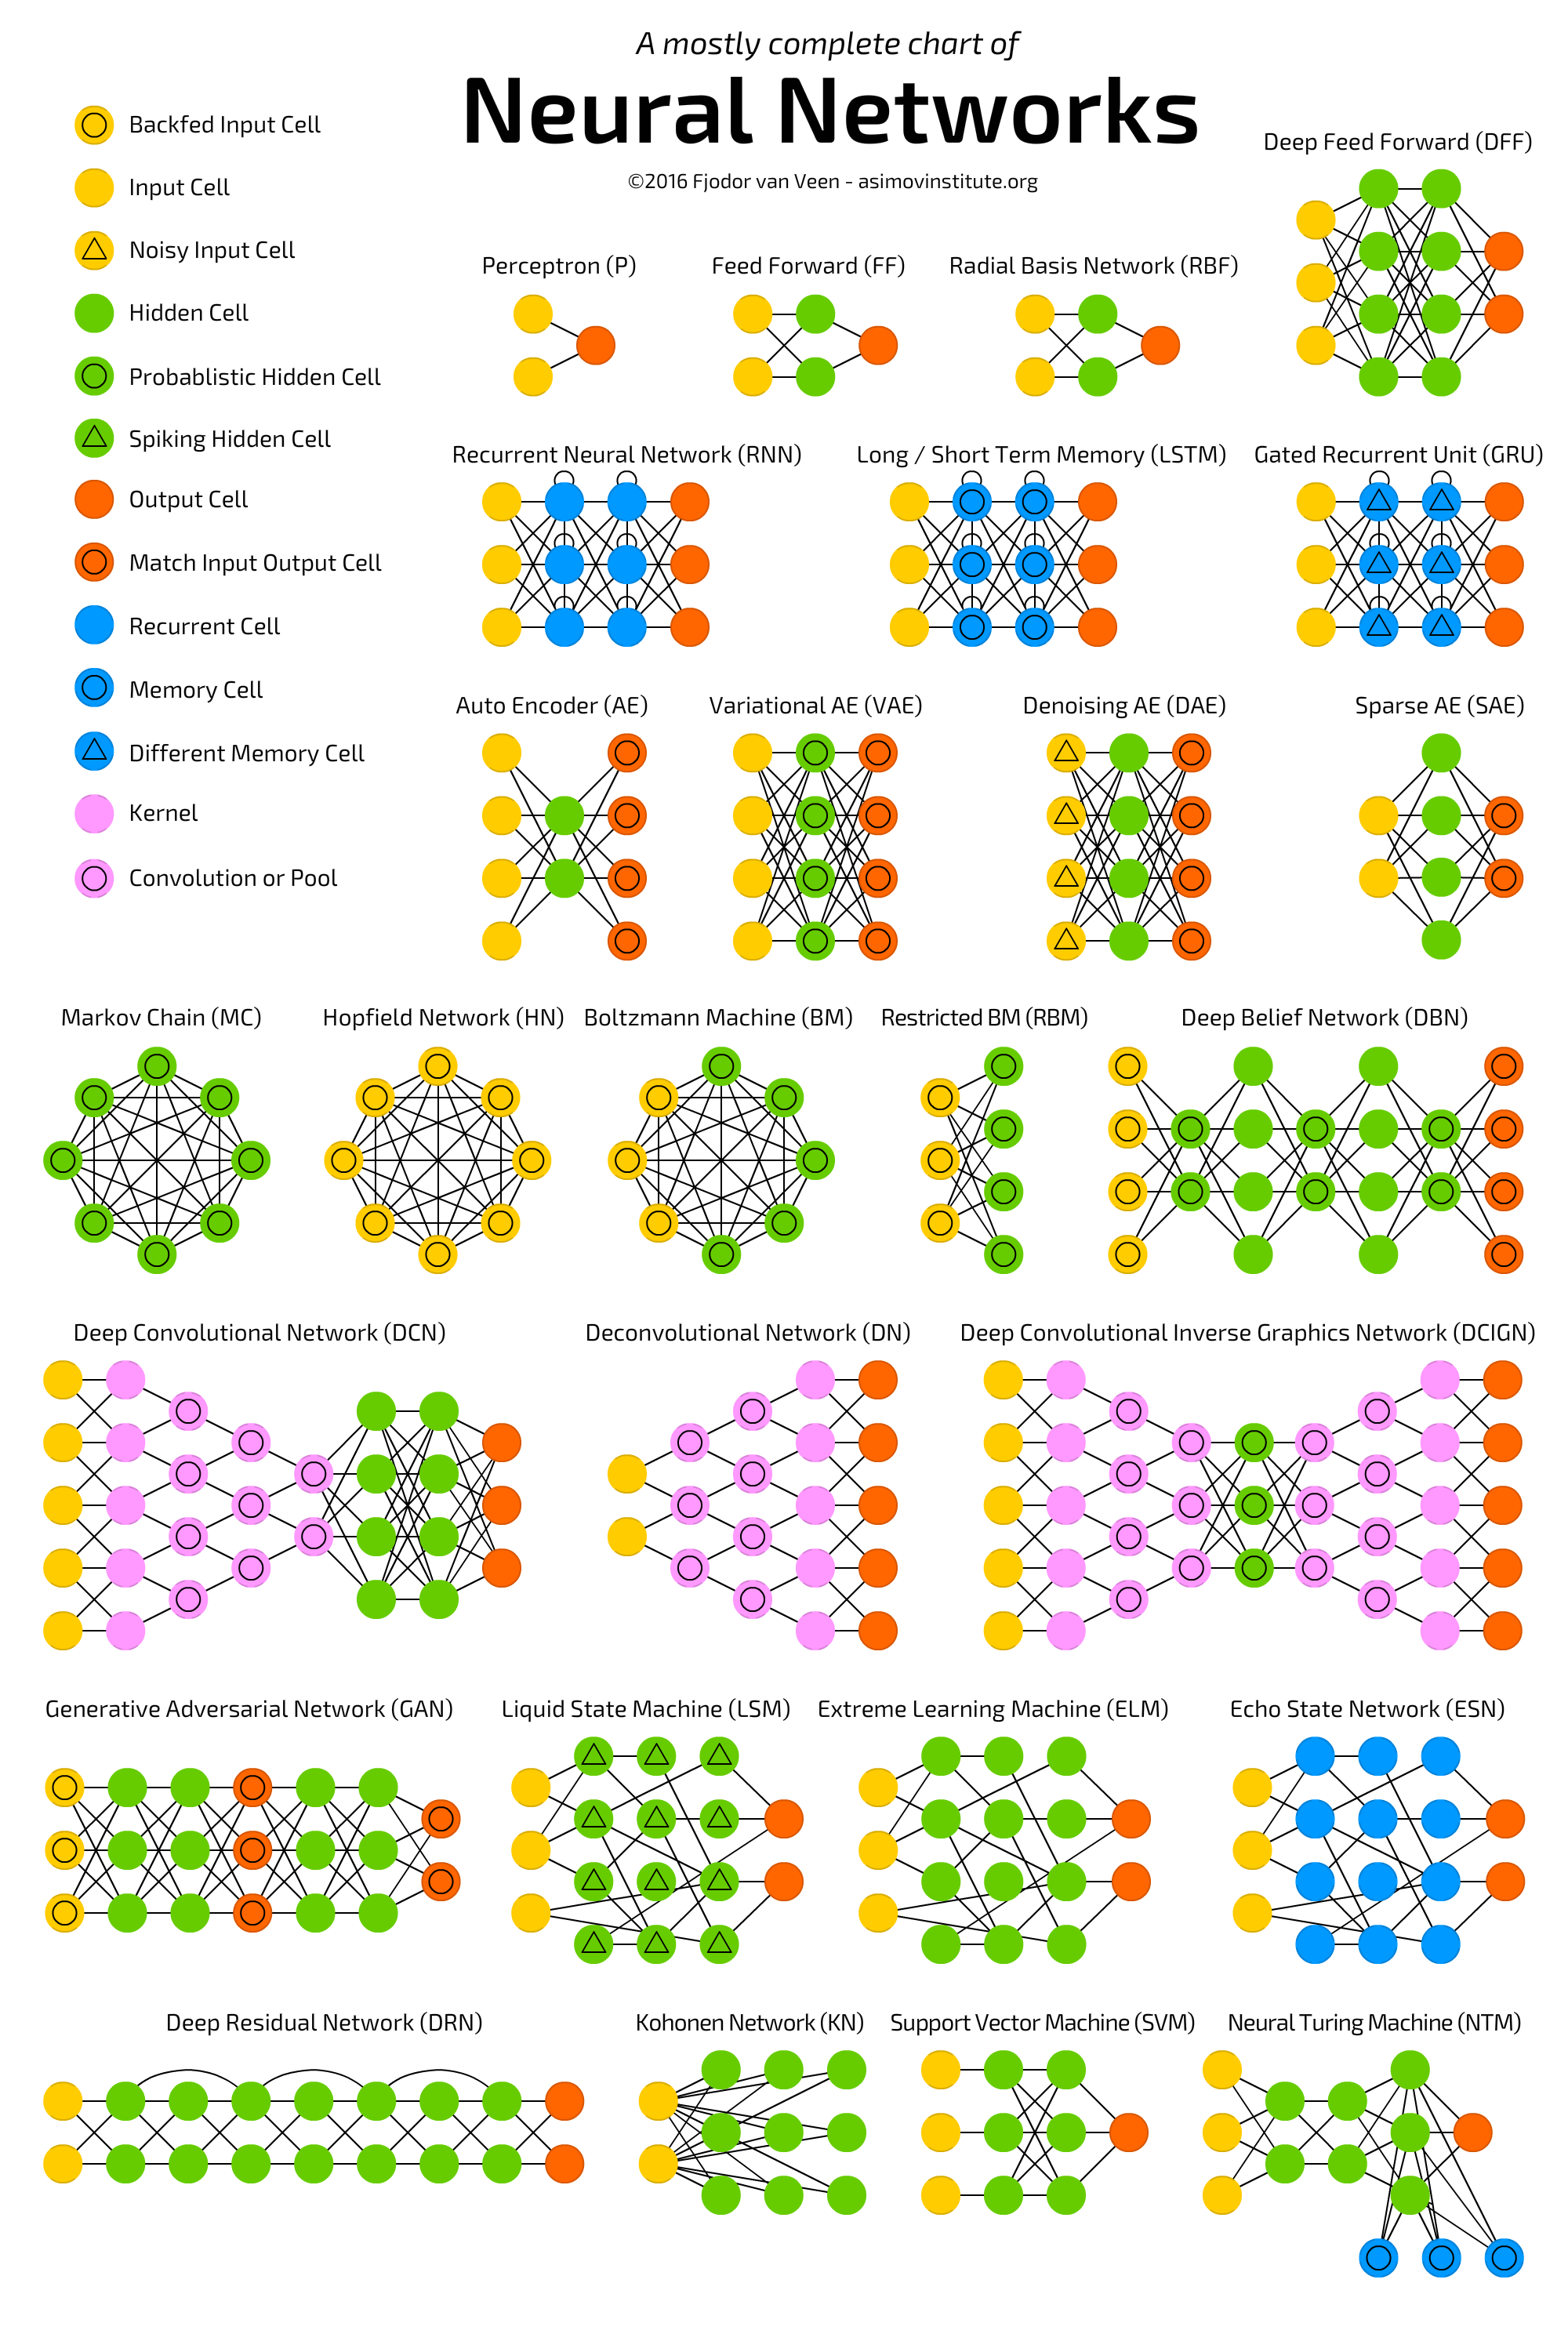
\includegraphics[width=0.75\textwidth]{types_of_NN.png}
%\captionsetup{width=0.7\linewidth}
%\caption{ \cite{types_of_NN_pic}}
\end{figure}
\begin{center}A guide to common types of neural networks, created by van Vleen \cite{types_of_NN_pic}.\end{center}
\newpage

\section{Types of Loss Functions}
\label{appendix:types_of_loss_functions}
\begin{figure}[ht]
\centering
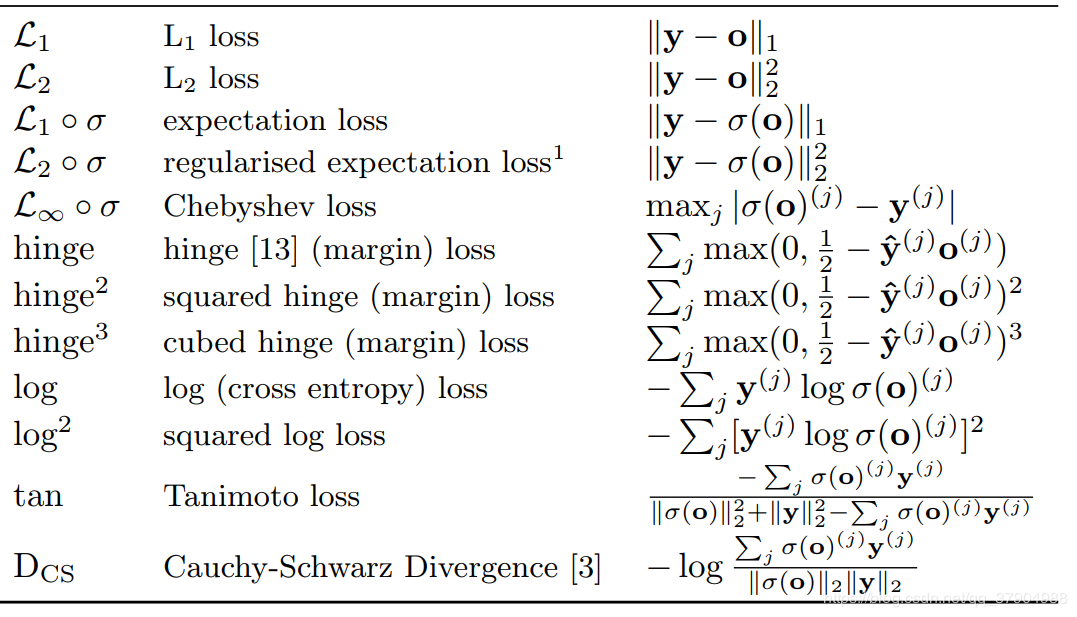
\includegraphics[width=0.8\textwidth]{loss_functions.png}
\end{figure}
\begin{center}A guide to loss functions, created by Janocha and Czarnecki \cite{loss_functions_paper}.\end{center}
\end{appendices}


%% TODO: get list of loss and activation functions and add them to appendix, then \ref them in the paper

%%%%%%%%% REFERENCES
\newpage
\printbibliography
\end{document}